%----------------------------------------------------------------------------------------
%	PACKAGES AND OTHER DOCUMENT CONFIGURATIONS
%----------------------------------------------------------------------------------------

\documentclass[fleqn,11pt]{SelfArx} % Document font size and equations flushed left

\usepackage{parskip}
\usepackage{microtype}
\usepackage{svg}
\usepackage{float}
\usepackage{placeins}
\usepackage[english]{babel} % Specify a different language here - english by default
\usepackage{listings}
\usepackage{fontspec}
\usepackage{hyperref}
\usepackage{amsmath}
\usepackage{makecell}
% \usepackage{lipsum} % Required to insert dummy text. To be removed otherwise
\setmainfont{TeX Gyre Termes}
%----------------------------------------------------------------------------------------
%	COLUMNS
%----------------------------------------------------------------------------------------

\setlength{\columnsep}{0.55cm} % Distance between the two columns of text
\setlength{\fboxrule}{1pt} % Width of the border around the abstract

%----------------------------------------------------------------------------------------
%	COLORS
%----------------------------------------------------------------------------------------

\definecolor{color1}{RGB}{124,0,0} % Color of the article title and sections
\definecolor{color2}{RGB}{150,150,150} % Color of the boxes behind the abstract and headings

%----------------------------------------------------------------------------------------
%	HYPERLINKS
%----------------------------------------------------------------------------------------

\usepackage{hyperref} % Required for hyperlinks
\hypersetup{hidelinks,colorlinks,breaklinks=true,urlcolor=color2,citecolor=color1,
  linkcolor=color1,bookmarksopen=false,pdftitle={Title},pdfauthor={Author}}

%----------------------------------------------------------------------------------------
%	ARTICLE INFORMATION
%----------------------------------------------------------------------------------------

\PaperTitle{
    HAMdetector: Combining information to detect HLA-associated mutations with a
    Bayesian regression model
} % Article title

\Authors{Daniel Habermann\textsuperscript{1}, ..., Daniel Hoffmann\textsuperscript{1}} % Authors
\affiliation{\textsuperscript{1}\textit{Bioinformatics \& Computational Biophysics, Faculty of Biology, University of Duisburg-Essen, 45117 Essen, Germany}} % Author affiliation
% \affiliation{\textsuperscript{2}\textit{Department of Chemistry, University of Examples, London, United Kingdom}} % Author affiliation
% \affiliation{*\textbf{Corresponding author}: john@smith.com} % Corresponding author

\Keywords{human leukocyte antigen system, HLA, multiple sequence alignment, escape mutations, 
  viral escape, Bayesian inference, sparsity, horseshoe, epitope prediction} % Keywords - if you don't want any simply remove all the text between the curly brackets
\newcommand{\keywordname}{Keywords} % Defines the keywords heading name

%----------------------------------------------------------------------------------------
%	ABSTRACT
%----------------------------------------------------------------------------------------

\Abstract{
  \\
  \textbf{Motivation} \\
  The human leukocyte antigen system (HLA) is of paramount importance to combat viral infections by presenting peptides on the cell surface via MHC I. Thus, CD8+ cytotoxic T-Lymphocytes exert a strong selection pressure towards virus variants that escape that immune recognition pathway, e.g. through point mutations that decreases binding of the respective peptide to MHC I. \\

  Reliably identifying HLA-associated mutations is important for understanding viral evolution, but experimental methods like binding assays are prohibitively expensive for large-scale use and fail to recognize other mechanisms of immune escape like proteasomal processing.

  One step in finding these mutations is through the statistical analysis of sequence data. However, existing methods are based on null hypothesis significance testing and do not make use of all the available information and therefore have unsatisfactory real-world performance. \\

  \textbf{Results} \\
  Here, we present a Bayesian regression model that is easily extensible to include information from different sources (e.g. epitope prediction software) and makes use of recent advances in Bayesian inference, e.g. by using a sparsifying prior. We show that including this kind of information improves predictive performance considerably over state-of-the-art methods. \\

  \textbf{Availability and Implementation} \\
  The source code of this software is available at \url{http://github.com} under a permissive MIT license. \\

  \textbf{Supplementary information} \\
  \href{https://google.com}{Supplementary data} are available at \textit{Bioinformatics} online. \\
}

%----------------------------------------------------------------------------------------
\begin{document}

\flushbottom % Makes all text pages the same height

\maketitle % Print the title and abstract box

{
  \hypersetup{linkcolor=black}
  \tableofcontents
}


\section{Introduction}

\subsection{The HLA system}

One way how the human immune system is able to recognize intracellular viral infections is through the human leukocyte antigen system\nolinebreak\cite{Germain1994}: In cells with active protein biosynthesis, proteins are continuously synthesized and also degraded by a process called proteasomal degradation, which cleaves proteins into linear peptides of varying length\nolinebreak\cite{Goldberg2002}.

A small subset of these peptides is presented on the cell surface via receptors called MHC class I (HLA-A, HLA-B and HLA-C in humans). The genomic region encoding for MHC I is known to be highly polymorphic, with more than 20000 different HLA alleles described today\nolinebreak\cite{Robinson2014}. The resulting gene products differ in their binding properties, which means that cells from different individuals present a highly diverse set of peptides on their surface.

Cytotoxic T cells are selected during maturation to only weakly bind to peptide/MHC I complexes when the peptide originated from proteins of the usual proteome, but might be able to strongly bind to complexes of MHC I with peptides which are  generated from of a viral protein\nolinebreak\cite{Murata2007}. Upon activation, T cells induce cytolytic activity and recruit other immune cells \nolinebreak\cite{Harty2000}.

\subsection{HLA escape}
In this way, the HLA system exerts strong selection pressure towards virus variants that escape T cell recognition\nolinebreak\cite{Borrow1997}, for example through a point mutation that results in reduced binding of an immunogenic peptide to MHC I or through a set of mutations that alters the viral protein in such a way that it is cleaved into different peptides that are not recognized by the host's T cell repertoire\nolinebreak\cite{Yewdell2002}.

The evolutionary events are complex and occur not only on the level of individuals, where a virus adapts to specific features of the host, but also on the population level, because HLA alleles differ in their frequency across geographic regions\nolinebreak\cite{Kawashima2009}. Upon transmission to a new host, HLA escape mutations can revert to their wild type, as HLA escape mutations are associated with a reduction in viral replicative capacity\nolinebreak\cite{Matthews2008}. Kawashima et al. \nolinebreak\cite{Kawashima2009} describe an escape mutation that is selected by HLA allele HLA-B*51, does not strongly affect viral replicative capacity, and therefore slowly enriches over time in Japan, where HLA-B*51 commonly occurs.

How quickly a given escape mutation is selected upon transmission in a host depends on the magnitude of the reduction in viral replicative capacity, on the strength of selection pressure, and also on the genetic background, e.g. some escape mutations require compensatory mutations which partly attenuate the negative impact on viral replicative capacity.

Studying HLA escape provides a unique opportunity to gain insight into viral evolution, on the host level, but also on the population level.
Unfortunately, identifying HLA escape mutations is difficult in practice.

\subsection{Identifying HLA-escape mutations}

There are several experimental methods available to study HLA escape: Recombinant MHC-I molecules can be used in binding assays. Upon complex formation with a peptide, a change in conformation can be detected with conformation-specific antibodies. This method is relatively fast, but only measures binding affinity of a peptide to MHC-I and does not account for antigen processing or immunodominance, which describes the observation that a peptide may be presented via MHC-I on the cell  surface, but does not induce an immune response.

An experimental setup that resembles the conditions in-vitro more closely but is also more time-consuming is to measure CD8+ T cell responses instead. This is usually done by stimulating peripheral blood mononuclear cells with prototype and variant peptides and measuring the secretion of IFN-\gamma{} by intracellular cytokine staining and fluorescence-assisted cell sorting.

To analyze CD8+ T cell responses against endogenously processed antigens, it is necessary to generate cell-lines stably expressing the antigen in question and adding antigen-specific CD8+ T cells. This method scales poorly as it requires transfection of cell lines and antigen-specific expansion of CD8+ T cells.

\subsection{Computational methods}

Because the currently available experimental methods do not scale well enough to analyze whole viral genomes, a useful strategy might be to use annotated sequence data to identify candidate HLA escape mutations that can then be verified experimentally.

As the selection pressure exerted by cytotoxic T cells depends on successful recognition of viral peptides on the cell surface, escape mutations are often HLA-allele specific and can therefore be detected as HLA-allele dependent footprints in sequence alignments of viral proteins\nolinebreak\cite{Moore2002}: At certain alignment positions, a replacement might be more frequently observed in sequences from hosts with a specific HLA allele than in  sequences from hosts without that HLA allele. By quantifying this difference for all replacement and HLA allele pairs, it is possible to identify replacements that are enriched in sequences coming from hosts with certain HLA alleles, and thus are likely to be HLA escape mutations.

One way of quantifying this enrichment is Fisher's exact test\nolinebreak\cite{Fisher1922}: For a given replacement \(R_{i}\) at alignment position \(i\) and HLA allele \(H\), a 2-by-2 contingency table is constructed containing the absolute counts of the number of sequences in the four possible categories  (\(R_{i}\), \(H\)), (\(R_{i}\), \(!H\)), (\(!R_{i}\), \(H\)) and (\(!R_{i}\), \(H\)), where \(!R_{i}\) denotes any replacement except \(R_{i}\), and \(!H\) denotes any HLA allele except \(H\).

Fisher's exact test is a conventional null hypothesis significance test (NHST) that generates p-values. In this case, the null hypothesis is that HLA allele \(H\) and  replacement \(R_{i}\) are independent, and the p-value is the probability of observing a deviation from independence that is at least as extreme as in the data at hand under the assumption that the null hypothesis is true.

Fisher's exact test has the advantage of being easy to apply\nolinebreak\cite{Budeus2016},  but also has several disadvantages that are outlined in Carlson et al.\nolinebreak\cite{Carlson2008}. The most striking one is that viral sequences share a common phylogenetic history, and,  therefore, treating sequences as independent and identically distributed samples may under- or overestimate effect sizes. In the context of hypothesis testing, this leads to increased false positive and false negative rates. 

Another issue of applying Fisher's exact test is that HLA class I loci are located in proximity on chromosome 6 and are therefore in linkage disequilibrium, which means that HLA alleles are not inherited completely independent of each other, i.e. inheritance of one HLA allele correlates with inheritance of another HLA allele. When using a statistical method that tests each HLA allele individually without considering the whole set of alleles present, spurious associations might occur: If HLA allele \(H_{1}\) is associated with an amino acid replacement \(R\), but \(H_{1}\) is in linkage disequilibrium with another allele \(H_{2}\), this also means that we observe an association between replacement \(R\) and \(H_{2}\), even in absence of any underlying escape mechanism.

Correlations can not only occur between HLA alleles, but also between replacements. This kind of codon covariation occurs for example in compensatory mutations that attenuate the negative impact of immune escape mutations. For instance, a compensatory mutation might lead to a conformational change in such a way that the mutated protein resembles the original wild type more closely.

Carlson et al. \nolinebreak\cite{Carlson2008} developed a method called  Phylogenetic Dependency Network that accounts for phylogenetic bias,  HLA linkage disequilibrium, and codon covariation and is based on null hypothesis significance testing.

\subsection{Issues with using p-values as a screening tool}

In addition to the aforementioned biological reasons why Fisher's exact test is  not suited for the analysis of sequence data, there are also more fundamental statistical issues that universally occur when using p-values as a screening tool\nolinebreak\cite{Amrhein2017}:

In the presence of small effect sizes and high variance between measurements, as  it is typically the case when working with biological data, statistically significant results can often be misleading and are likely to be in the wrong direction (a so-called type S error) or greatly overestimate an effect (a so-called type M error)\nolinebreak\cite{Gelman2014}. This problem has recently been widely appreciated in the literature in the context of the current \glqq replication crisis\grqq{}, which describes the circumstance that scientific claims with seemingly strong statistical evidence fail to replicate\nolinebreak\cite{Ioannidis2005}.

Another issue that occurs when using p-values as a screening tool is the problem of multiple comparisons. When applying a statistical test, the probability  of  obtaining a statistically significant result increases with each additional test, even in absence of any real effect. When using p-values as a filter, it is therefore likely to obtain significant effects that are in fact not real. To circumvent this problem, a common strategy is to control the false discovery rate, which is the expected proportion of false positives\nolinebreak\cite{Benjamini1995}. These adjustment procedures have the problem that, when performing many of such comparisons, none but the very largest effects remain.

Instead of performing many hypothesis tests and trying to adjust for them, we instead prefer to fit a single, multilevel model that contains all comparisons of interest. When using multilevel models, the problem of multiple comparisons can disappear entirely and  also yield more valid estimates\nolinebreak\cite{Gelman2012}.

\section{Material and methods}

When possible, we choose to fit Bayesian models. By using prior information, adding problem-specific structure and partial pooling, the accuracy of estimates can often be noticeably improved\nolinebreak\cite{Gelman2010}. Prior information does not necessarily mean to use external data, even a rough idea about the expected magnitude of estimates is often surprisingly effective.

Additionally, Bayesian statistics provides an accessible way to test models: By comparing data generated under the model's assumptions to the actually observed data, it is possible to identify important aspects of the dataset that the models fails to capture and subsequently improve the model until it is consistent with the observed data\nolinebreak\cite{Gabry2019}.

In the context of identifying HLA-associated mutations we propose to improve existing methods by the following additions, which can be broadly divided into  additional information and model structure:
\subsection*{Additional information}

  \textit{Binding affinity prediction}

    HLA-associated mutations are expected to lie more frequently in regions of known epitopes. There are vast experimental binding affinity data available of different peptides and MHC I molecule pairs, and there are well-established computational methods that use these data to extrapolate HLA binding for untested peptides. We show that, by including the outcome of these computational tools as input for a probabilistic model, the prediction of HLA-associated mutations can be improved.

  \textit{Antigen processing prediction}
  
    Similarly, there are also HLA-allele independent effects like antigen processing that influence presentation on MHC I. Second generational tools like MHCFlurry 2.0 use both binding affinity and antigen processing data to improve epitope prediction. For our tool HAMdetector, we use the output of MHCFlurry to benefit from this binding affinity and antigen processing data in order to predict HLA-associated mutations.

\subsection*{Model structure}

  \textit{Sparsity-inducing priors}
  
  Recent advantages in Bayesian inference include so-called sparsity-promoting priors. Sparsity-promoting priors convey the a priori expectation that most coefficients in a regression model are close to 0. This assumption also applies to HLA-associated mutations, because the number of epitopes that are restricted by a given HLA allele is typically small compared to the number of all possible epitopes. If no epitope spanning a given alignment position is presented on the MHC I molecule, any association between a replacement and the respective HLA allele  is likely to be due to random variation alone (or HLA linkage disequilibrium).
  
  It has been shown that using a sparsity-promoting prior when non-zero coefficients are sparse can drastically improve predictive performance, because the model is better able to differentiate between signal and noise.

  We show that a simple logistic regression model with a sparsity-promoting prior on the regression coefficients for the HLA alleles alone already performs roughly on-par  with the much more elaborate Phylogenetic Dependency Network approach from Carlson et al. when using the fraction of identified escapes that lie in known HLA epitopes as a benchmark.

  \textit{Partial pooling of 4-digit HLA alleles}
  
  It has recently been appreciated that binding specificities can vary drastically across  HLA alleles from the same allele group, e.g. between HLA-B*51:01 and HLA-B*51:03. For predicting HLA associated mutations, there has consequently been a shift to use 4-digit resolution data whenever available. This is not without downsides however, because overall, binding specificities are more similar for alleles in the same group, and, therefore, treating them as completely separate might unnecessarily fragment the available data.

  In Bayesian statistics, it is not required to chose one extreme or the other: Instead of either treating all HLA alleles from the same allele group as identical or as completely separate, partial pooling of the estimates allows something in between: By partial pooling, estimates do share some information across each other, but they are also allowed to vary if necessary.

  In the context of our model this means that observing a relevant association between a replacement and an HLA allele also makes the model more inclined to estimate relevant associations between that replacement and all other alleles from that allele group. The degree of this partial pooling can be estimated from the data, so if we do observe strong similarity of HLA alleles in a given allele group the estimates are more influenced by each other than if they do not.

\section{Implementation}

\subsection*{Model backbone}

We chose a logistic regression model as a backbone for two reasons: First, because it is easily extensible and secondly, because the coefficients are interpretable as expected increases on the log-odds scale, identical to the familiar interpretation of standard logistic regression models.
We also chose to fit the model in a Bayesian fashion using Stan, mostly because it allows us to make use of the hierarchical structure in the data and the possibility to use posterior predictive checks as a way of model checking.
Consider the following notation:

\begin{align}
  y_{ik} & \sim \text{bernoulli}(\theta_{ik}) \\
  \theta_{ik} & = \text{inv\_logit}(\beta_{0_{k}} + \sum_{j=1}^{D} X_{ij}\beta_{\text{HLA}_{jk}})
\end{align}, 

where \(y_{ik}\) is the binary encoded observation at sequence \(i\) for replacement \(k\), \(\theta_{ik}\) is the estimated probability that we observe replacement \(k\) in sequence \(i\), \(X_{ij}\) is 1 if sequence \(i\) is annotated with HLA allele \(j\) and 0 otherwise, \(\beta_{\text{HLA}_{jk}}\) is the HLA regression coefficients for HLA allele \(j\) at replacement \(k\), \(D\) is the number of HLA alleles in the dataset, and \(\text{inv\_logit}\) is the logistic link function. Note that, if we observe N different amino acid states at a certain alignment position, each of those are considered in turn to be the “replacement”.

The regression coefficients \(\beta_{\text{HLA}_{jk}}\) are the main focus of interest, as they quantify the association between the occurrence of replacement \(k\) and each of the observed HLA alleles. They are in units of log-odds, so a regression coefficient of somewhere around 2 means that when comparing sequences with and without that particular HLA allele, the log-odds of observing replacement \(k\) in presence of that HLA allele is increased by 2.

Reasoning about coefficients on the log-odds scale can sometimes be unintuitive. A useful approximation to interpret logistic regression coefficients on the probability scale is the so-called divide-by-4 rule, which means that a regression coefficient of 2 corresponds to an expected increase on the probability scale of about 2/4 = 50\%. 

\subsection*{Including phylogeny}

One problem that occurs when analyzing sequence data is that species share a common phylogenetic history. Standard statistical methods usually assume samples to be independent and identically distributed, which may lead to wrong conclusions when this assumption is strongly violated.
In the context of identifying HLA associations, Bhattacharya et al.\cite{Bhattacharya2007} demonstrated the importance of correcting for the phylogenetic structure.
There are many approaches described in the literature for phylogenetic regression for binary dependent variables (see \cite{Ives2014}), where the most popular approach is to estimate an additional multivariate normally distributed intercept, where the covariance matrix is based on the branch lengths of a given phylogenetic tree \cite{Ives2009}.

This approach showed to be too computationally expensive to include in our model, so we chose a strategy that is similar to the one in Carlson et al. \cite{Carlson2008} for the Phylogenetic Dependency Network:

Consider a phylogenetic tree \(\Psi\) obtained from standard maximum likelihood methods for a given multiple sequence alignment. We are interested in estimating \(P(y_{ik}=1|\Psi)\), that is, the probability of observing the replacement \(k\) in sequence \(i\) based on the underlying phylogenetic model.
A quantity that can be readily computed using phylogenetic software like RAxML-NG~\cite{Kozlov2019} is \(P(\Psi|y_{ik}=1)\). For this, we keep the tree topology fixed, annotate the tree with the binary observations \(y\) at its leaves and optimize the branch lengths. \(P(\Psi|y_{ik}=1)\) is then the likelihood of the annotated phylogenetic tree. We can then use Bayes' rule to invert that conditional probability by additionally computing \(P(\Psi|y_{ik}=0)\), which is done by altering the annotation for sequence \(i\) and keeping all other observations constant.

In order to check if the inferred probabilities \(P(y_{ik}=1|\Psi)\) faithfully reflect the observed data we use calibration plots (see fig.~\ref{fig:phylogeny-calibration}). All observations are binned according to their inferred probability \(P(y_{ik}=1|\Psi)\). If these probabilities are calibrated correctly, we expect that in a group of observations with an inferred probability \(P(y_{ik}=1|\Psi)\) of around x\% we really do observe \(y_{ik}=1\) around x\% percent of the time.

\begin{figure}[!ht]
  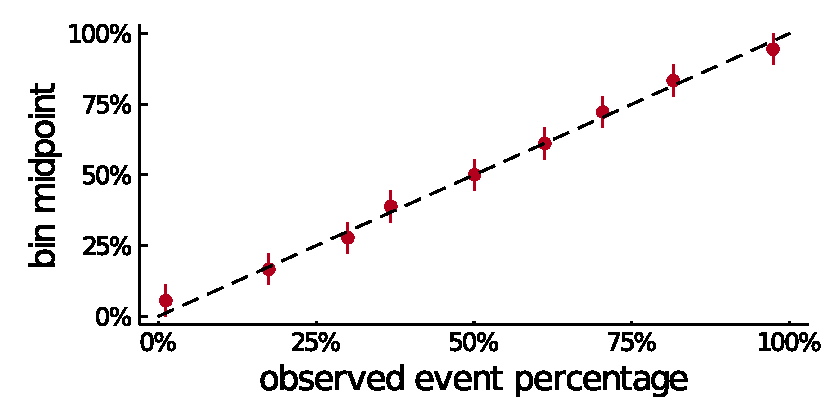
\includegraphics[width=1\linewidth]{plots/phylogeny_calibration.pdf}
  \caption{Calibration plot for the HBV dataset. For a description of all datasets used in this study see section~\ref{sec:results}. Calibration plots for the other datasets are shown in the appendix.
  All observations are first sorted by increasing estimated probability \(P(y_{ik}=1|\Psi)\) and then grouped into \(n\) bins.
  For each bin, the fraction of observations with \(y_{ik}=1\) (observed event percentage) is compared to the midpoint of each bin (the value in the center between the lowest and highest probability). The error bars show the cutpoints for each bin. If the probabilities are calibrated correctly, each dot is supposed to scatter closely around the diagonal line.}
  \label{fig:phylogeny-calibration}
\end{figure}

The estimated probabilities are then included in the model as additional intercepts:

\begin{equation}
\begin{aligned}
  y_{ik} & \sim \text{bernoulli}(\theta_{ik}) \\
  \theta_{ik} & = \text{inv\_logit}(\beta_{0_{k}} + \gamma~\text{logit}(P(y_{ik}=1|\Psi)) \\ + \sum_{k=1}^{D}X_{ik}\beta_{\text{HLA}_{jk}})
\end{aligned}
\end{equation}

The logit transform is used because is cancels out with the logistic link function. This means that the phylogeny information acts as a baseline in absence of any HLA effects. Note that we also include an additional parameter \(\gamma\), that is constrained to be positive. This helps because the inferred probabilities \(P(y_{ik}=1|\Psi)\) might not necessarily reflect the true underlying phylogenetic signal, for example because the phylogenetic tree does not match the observed data well enough.

A straight-forward extension of our model would be to also account for these sources of uncertainty, for example by using a Bayesian method to estimate a posterior distribution over possible tree topologies. The uncertainty over the tree topology and the underlying parameters of the phylogenetic model would then propagate into uncertainty of the estimated probabilities \(P(y_{ik}=1|\Psi)\). However, in order to not increase the runtime of the model further we  use standard maximum likelihood estimates and then include these in a way that allows for measurement error.

\subsection*{Including HLA linkage disequilibrium and codon covariation}

The other two important confounding effects that are recognized in Carlson et al.\cite{Carlson2008} are HLA linkage disequilibrium and codon covariation.
HLA linkage disequilibrium describes the observation that HLA alleles that lie in proximity to each other on the chromosome are also more likely to be inherited together. When using a statistical method that evaluates each HLA allele individually, this may lead to spurious associations: If some HLA allele \(X\) is associated with replacement \(k\), and HLA allele \(Y\) often co-occurs with HLA allele \(X\), this means that we also identify an association between HLA allele \(Y\) and replacement \(k\).

This association is correct in a statistical sense, but if the purpose of the model is to identify sites under HLA-mediated selection pressure, these associations due to linkage disequilibrium are most likely unwanted.

Note that these spurious associations only occur when testing each HLA allele individually. In a regression model where all HLA alleles of a sample are evaluated at once, the marginal poster distributions for correlated predictors become broader to accurately reflect that the model is unable to discern which of these predictors explain the observed association with a replacement.

We do not currently account for codon covariation in our model, as we are interested in identifying all HLA associated mutations (which include for example compensatory mutations). The general structure of the model, in particular the sparsity assumption introduced in section~\ref{sec:sparsity},would allow adding codon covariation by adding all other codons as additional predictors. This would generally not be possible in a frequentist setting because the predictor matrix would become singular and the inverse does not exist. 

\subsection*{Including sparsity assumptions} \label{sec:sparsity}

One of the recent advances in Bayesian inference is the development of special prior distributions which can be used to give models additional useful properties. An example of these special prior distributions are the so-called sparsity-inducing priors, which can be used to convey the assumption that most of the predictors in a regression model are not associated with the outcome and are therefore 0.

In the context of identifying HLA associations we expect most of the HLA coefficients to be very close to 0, as a given alignment position is typically only restricted by none or few HLA alleles.
This is important prior knowledge that should be incorporated in the model.
Adding this sparsity assumption can lead to better inferences, because the uncertainty of the non-relevant HLA regression coefficients does not propagate further and therefore the model is able to better discern signal from noise.

There are a variety of different sparsity-promoting priors with slightly different properties. They share the common structure of placing most probability mass very close to 0, with large to tails to accommodate the non-zero coefficients.
For our model, we use a so-called horse prior~\cite{Carvalho2010}, which is defined as a scale-mixture of gaussians:

\begin{equation}
  \begin{aligned}
    \beta_{jk} &\sim \text{Normal}(0, \tau^{2}\lambda^{2}_{jk}) \\
    \lambda_{jk} &\sim \text{Cauchy}^{+}(0, 1) \\
    \tau &\sim \text{Cauchy}^{+}(0, \tau_{0})
  \end{aligned}
\end{equation},

where \(\beta_{jk}\) are the regression coefficients, \(\tau\) is the so-called global shrinkage parameter, \(\lambda_{jk}\) are the so-called local shrinkage parameters and \(\text{Cauchy}^{+}\) is the positively constrained Cauchy distribution.

Intuitively speaking, the global shrinkage parameter \(\tau\) is typically very small and shrinks most of the regression coefficients to 0, whereas the local shrinkage parameters can occasionally be very large to allow some coefficients to escape that shrinkage.

A useful addition to the horseshoe prior is given in Piironen et al.\cite{Piironen2017}, which describes a way to choose the parameter governing the overall degree of sparsity \(\tau_{0}\) based on the expected number of non-zero coefficients. 

For our HLA model, we utilize an extension to the horseshoe prior called the regularized horseshoe prior~\cite{Piironen2017}, which also provides some regularization for the non-zero coefficients. This is particularly useful for logistic regression models, as some shrinkage helps to deal with issues of separability and collinearity.

Figure~\ref{fig:horseshoe-comparison} shows a comparison of marginal posteriors for regression coefficients with and without horseshoe prior.

The improvement of the logistic regression model with the horseshoe prior is a considerable improvement over a standard logistic regression model (see section~\ref{sec:results}. In our benchmark, the horseshoe prior alone is even shown to be more effective than a model without horseshoe prior but with phylogeny included.

\begin{figure}
  \label{fig:horseshoe-comparison}
\end{figure}

\subsection*{Including epitope prediction software}

There is vast experimental data on epitope binding motifs available, e.g. through the use of mass spectrometry~\cite{Hunt1992}. Epitope prediction software like MHCFlurry~\cite{ODonnell2020} use these data to extrapolate MHC I binding for new, untested peptides.
As HLA-associated mutations are much more likely to lie in epitopes (e.g. because of selection pressure to escape MHC I binding), using epitope prediction software can provide valuable external data for identifying HLA-associated mutations.

For our model, we use MHCFlurry 2.0 for binding prediction, as it does not only predict HLA binding but also predicts antigen processing. For this, we create an input matrix of dimensions \(R\times D\), where R is the number of evaluated replacements and D is the number of observed HLA alleles in the dataset. The elements of this matrix are binary encoded and contain a 1 if that position is either expected to be inside a predicted epitope or related to antigen processing, and 0 otherwise. Given an amino acid sequence, MHCFlurry 2.0 provides a list of possible epitopes (9-13 mers) and HLA allele pairs and calculates a rank based on comparisons with random epitope and HLA pairs. For the binarization we use a rank threshold of 0.2\% (as suggested by MHCFlurry).

We typically try to avoid thresholds whenever possible, but in this case we deemed it to be preferable to including the predicted binding affinities, as we expected the binary values to be more reliable than the predicted numeric values.
Note that the output of these epitope prediction tools may be imprecise or even wrong, but by including it as an input for a probabilistic model, the model is able to learn how much to trust this data if parameterized in a way to allow for measurement error.

We use epitope prediction as information about the expected degree of sparsity, i.e. when knowing a certain position is restricted by a certain HLA allele, we expect that this HLA allele is more likely to be associated with the replacement than the other HLA alleles.
This can be reflected by increasing the scale of the local shrinkage parameters \(\lambda_{jk}\):

\begin{equation}
  \begin{aligned}
    \lambda_{jk} &\sim \text{Cauchy}^{+}(0, \text{exp}(Z_{jk}\beta_{\text{epi}})) \\
    \beta_{\text{epi}} &\sim \text{Normal}^{+}(1, 2)
  \end{aligned}
\end{equation},
 
where \(Z_{jk}\) is 1 if HLA allele \(j\) is predicted to restrict the alignment position corresponding to replacement \(k\) or is associated antigen processing and 0 otherwise.
The parameter \(\beta_{\text{epi}}\) governs the increase in scale of the  corresponding local shrinkage parameters. The larger the estimated values of \(\beta_{\text{epi}}\) are, the more likely it is to see non-zero regression coefficients for these HLA alleles.

\subsection*{Full model specification}

The full specification of the model is given by:

\begin{equation}
  \label{eq:full}
  \begin{aligned}
    y_{ik} &\sim \text{bernoulli}(\theta_{ik})\\
      \theta_{ik} &=
        \text{inv\_logit}(\beta_{0_{k}} + \gamma_{k}\text{logit}(P(y_{ik}=1|\Psi))\\
        \hspace{-6cm} &~~~~ +\sum_{k=1}^{D}X_{ij}\beta_{\text{HLA}_{jk}}) \\
    \beta_{0_{k}} &\sim \text{Normal}(0, 100^2)\\
    \gamma_{k} &\sim \text{Normal}(\mu_{\text{phy}}, \sigma_{\text{phy}}^2)\\
    \mu_{\text{phy}} &\sim \text{Normal}(1, 1)\\
    \sigma_{\text{phy}} &\sim \text{Normal}^{+}(0, 0.5)\\
    \beta_{\text{HLA}_{jk}} &\sim \text{Normal}(0, \tau^{2}\tilde{\lambda}^{2}_{jk})\\
    \tilde{\lambda}^{2}_{jk} &= \frac{c_{k}^{2}\lambda_{jk}^{2}}{c_{k}^{2} + \tau^{2}\lambda_{jk}^{2}} \\
    c_{k}^2 &\sim \text{Inv-Gamma}(3.5, 3.5)\\
    \lambda_{jk} &\sim \text{Cauchy}^{+}(0, \sigma_{j}^2\text{exp}(Z_{jk}\beta_{\text{epi}}))\\
    \tau &\sim \text{Cauchy}^{+}(0, \tau_{0})\\
    \tau_{0} &= \frac{2}{D-2}\frac{2}{\sqrt{N}}\\
  \end{aligned}
\end{equation}

The full model specification includes some aspects that were not covered in the previous sections. In particular, the parameters \(\gamma_{k}\) are modelled hierarchically, which allows information to be partially pooled across replacements. However, the model would also work reasonably well with just a single global parameter \(\gamma\). All other additions (\(\tilde{\lambda}_{jk}^{2}\) and \(\tau_0\)) are explained in detail in \cite{Piironen2017}. Briefly, the addition of  \(\tilde{\lambda}_{jk}^{2}\) allows some regularization for the non-zero coefficients and the parameterization of \(tau_{0}\) allows to place a prior on the expected number of non-zero coefficients.

All models were implemented in Stan. The Stan code is available online in two versions: One optimized for readability and one optimized for speed by utilizing Stan's multithreading and GPU capabilities.
A Julia\cite{Bezanson2017} package is available to run the model on custom data. Due to restrictions of dependencies (MHCFlurry and raxml-ng), HAMdetector is only available on Linux. We additionally provide Docker images to easily run the model on any operating system in a containerized environment, assuming Docker is installed. 

\subsection*{Prior justification}

Prior distributions are labeled with an asterisk in equation~\ref{eq:full}. They are meant to be weakly informative, which means that the goal is to provide some modest amount of shrinkage while still allowing for large absolute values given enough support by the observed data. One exception to this are the intercepts \(\beta_{0_k}\), which are essentially flat because they are well identified by the data alone.

The hierarchical mean and standard deviation of the phylogeny coefficients \(\gamma_{k}\) are chosen to place most probability mass at values of \(\gamma_{k}\) of around 1. In the absence of any HLA effects, a parameter value of 1 would mean that the estimate for the probability of observing replacement \(k\) is identical to the probability based on the phylogenetic model. Intuitively speaking, We therefore treat the phylogeny as a baseline and any observations that cannot be attributed to phylogeny are attributed to the HLA alleles or noise.

The prior on \(c_{k}^{2}\) implies a Student-t prior with 7 degrees of freedom and a scale of 1 on HLA regression coefficients \(\beta_{\text{HLA}_{jk}}\) that are estimated to be away from 0. A Student-t prior with these parameters is a reasonable default choice for logistic regression models. The theoretical justification behind this regularized variant of the horseshoe prior is explained in detail in\cite{Piironen2017}.

The value of \(\tau_{0}\) is chosen to imply 2 effective non-zero HLA regression coefficients per replacement. The rationale behind this parameterization is again outlined in\cite{Piironen2017}. The value of 2 is approximately based on available HIV epitope maps. Please note that this is only an approximate statement about the general magnitude, i.e. we would expect maybe a couple of HLA alleles to be associated with a single replacement, but not 20 or more.
The model is also parameterized in a way that assumes an equal degree of sparsity across all alignment positions a priori. We also tried to model \(\tau\) hierarchically, but observed sampling issues due to the resulting unfavorable geometry of the posterior.

\section{Results}

To show that our model works well in different real-world scenarios, we run versions of our model on several datasets:

\begin{itemize}
  \item A large HIV dataset consisting of X sequences, that were kindly provided by X and were also used in the Phylogenetic Dependency Network study~\cite{Carlson2008}.
  \item A set of 351 HIV sequences mostly spanning the Pol gene from the Arevir database~\cite{Roomp2006}
  \item A set of 544 Hepatitis-B-Virus sequences that were kindly provided by Jörg Timm.
  \item A set of 104 Hepatitis-D-Virus sequences that were kindly provided by Michael Roggendorf
  \item A set of 41 HIV sequences that were kindly provided by Rongge Yang
\end{itemize}

For all sequences, we applied the following data preparation steps:

\begin{enumerate}
  \item For each dataset, the sequences were split into subsequences, either by protein or gene.
  \item If not already present in this format, sequences were translated into their amino acid representation.
  \item RAxML-NG~\cite{Kozlov2019} version 1.0.0 was used to generate a maximum likelihood phylogenetic tree for each gene/protein using the \texttt{--model GTR+G+I} option with all other parameters set to default values.
\end{enumerate}

In order to evaluate each building block of HAMdetector, we applied 4 different Bayesian models to each dataset, each of which includes the previous model as a special case:
A standard logistic regression model, a logistic regression model with horseshoe prior, a model additionally including phylogeny and the full model with horseshoe prior, phylogeny and epitope prediction.
As a comparison to existing methods, we also applied Fisher's exact test and the Phylogenetic Dependency Network.

\subsection*{Convergence diagnostics}

For all the Bayesian models, Markov Chain Monte Carlo sampling was done using Stan. All model fits showed no signs of inference issues. In total, 4 different chains with 2000 samples each were drawn from the posterior. The effective sample size for all model parameters exceeded 500, R-hat convergence diagnostic values were below 1.01 in all cases.

\subsection*{Posterior predictive checks}

Bayesian modelling allows a simple yet effective strategy to test models: By simulating data under the model's assumptions and then comparing simulated and observed data, model misspecifications can be identified and highlight possible model improvements.

Here, we compare the calibration of the posterior predictive probability of observing the replacement to the actual observed data using calibration plots.
The plots are similar to the one showed in figure~\ref{fig:phylogeny-calibration} but this time do not evaluate the probabilities based on the phylogenetic model alone, but show the calibration of the posterior predictive probabilities based on the full model.

An example calibration plot of the AMdetector model on the Core protein sequence data of the HBV dataset is shown in figure~\ref{fig:calibration}. Plots for the other models and datasets are shown in the supplementary.

\begin{figure}[!ht]
  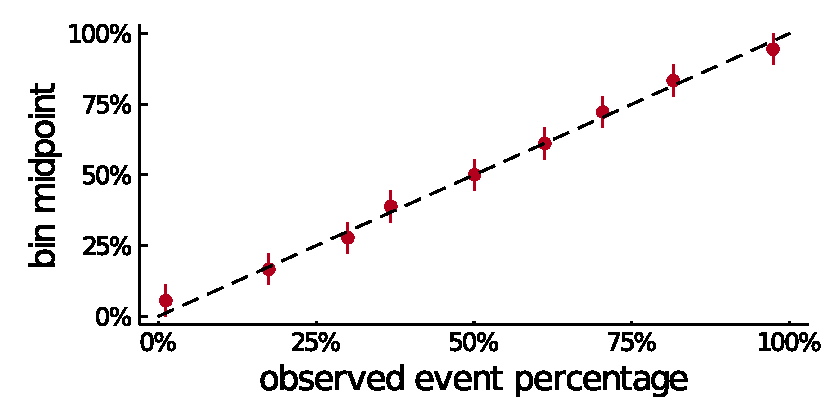
\includegraphics[width=1\linewidth]{plots/phylogeny_calibration.pdf}
  \caption{Calibration plot for the HBV dataset. Calibration plots for the other datasets are shown in the appendix.
  All observations are first sorted by increasing estimated probability \(P(y_{ik}=1)\) and then grouped into \(n\) bins.
  For each bin, the fraction of observations with \(y_{ik}=1\) (observed event percentage) is compared to the midpoint of each bin (the value in the center between the lowest and highest probability). The error bars show the cutpoints for each bin. If the probabilities are calibrated correctly, each dot is supposed to scatter closely around the diagonal line.}
  \label{fig:calibration}
\end{figure}

\subsection*{Comparison to a list of known epitopes}

When testing models, we prefer to evaluate them on real-world data whenever possible. 
However, comparing against real-world data is not straight forward when identifying HLA-associated mutations, because if a tool identifies an HLA-associated mutation which is not yet documented, this could be either because it is a false positive, or a yet unknown HLA-associated mutation that has not been documented before. 
Also, viewing every non-identified HLA-associated mutation that is listed in the literature as a false negative is not correct either, because documented escape mutations do not necessarily have to show in a sequence alignment.
A third issue when comparing models is that HLA-associated mutations are not necessarily binary, so the true positive / false negative framework does not work as well.

To circumvent these issues and still compare against real-world data, we chose the following strategy:
For each model, all evaluated replacements are ranked by decreasing confidence of being an HLA associated mutation. That is, for Bayesian models we calculate the probability of the corresponding regression coefficient exceeding zero \(P(\beta_{HLA} > 0)\), for Fisher's exact test we sort HLA allele - replacement pairs by increasing p-values and for the Phylogenetic Dependency Network, we rank the associations by increasing q-values.
Then, a list of known epitopes is used to create a plot of the cumulative number of replacements inside the boundary of a known epitope vs the corresponding rank. The underlying assumption for this kind of model check is that we expect to see an enrichment of replacements that lie inside the region of known epitopes and that this enrichment is stronger for better performing models.

\begin{figure}[ht!]
  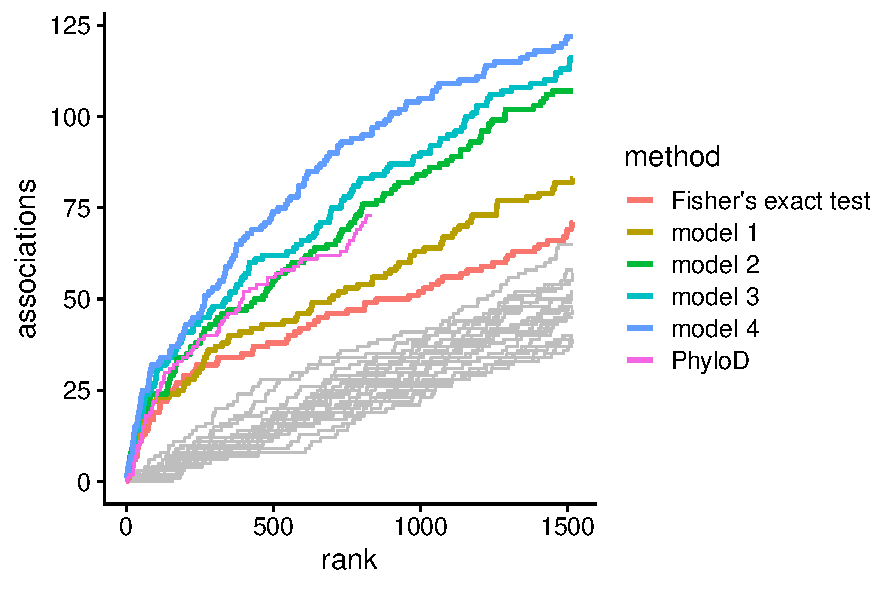
\includegraphics[width=1\linewidth]{plots/comparison.pdf}
  \caption{Number of associations inside the boundary of known epitopes vs. rank. For each model, the pairs of HLA alleles and replacements are sorted by decreasing confidence of being an HLA associated mutation. Then, each replacement is compared to a list of known epitopes and a line of the cumulative number of associations inside known epitopes vs. the current rank is plotted for each model. Better performing models are expected to have an enrichment of associations that are inside of known epitopes. 
  PhyloD: Phylogenetic Dependency Network, Model 1: simple logistic regression model with broad Student-t priors, Model 2: logistic regression model with horseshoe prior, Model 3: logistic regression model with horseshoe prior and phylogeny, Model 4: Full model with epitope prediction. The thin gray lines denote random permutations of the list of HLA allele - replacement pairs and act as a baseline.}
  \label{fig:comparison}
\end{figure}

Figure~\ref{fig:comparison} shows a comparison of different models on the HBe protein of the HBV dataset. Plots for all other datasets are shown in the Appendix, but show very similar patterns to the one shown here.

Unsurprisingly, all models show a strong enrichment of HLA-associated mutations compared to a randomly permutated list of HLA allele - replacement pairs (gray lines). Fisher's exact test performs about as well as the simple logistic regression model, as from a statistical perspective, they are both very similar.
The horseshoe prior alone is a drastic improvement over Fisher's exact test and the logistic regression model with non-sparsifying priors, even though it does not include any external information. The benefit comes from including the assumption that most regression coefficients are expected to be very close to 0.
The logistic regression model with horseshoe prior works roughly as well as the Phylogenetic Dependency Network, which includes much more information.
Note that the line for the Phylogenetic Dependency Network is shorter because it only outputs associations with a q-value lower than 0.2 by default.

The remaining models are ranked in order of the number of additional features they include. Additionally including phylogeny is a small improvement over the model with the horseshoe prior, while adding epitope prediction shows to larger drastic improvement.
Note that this model only uses epitope *prediction* software and does not utilize any information of experimentally confirmed epitopes. These are only used for model evaluation. Therefore, our method even works in absence of any experimental epitope information.

\subsection{Leave-one-out cross-validation}

In addition to testing the model against experimentally validated epitopes, we also perform leave-one-out cross-validation. While the comparison against known epitopes compares inferences of the regression coefficients, leave-one-out cross-validation compares different models in regard to their predictive performance, i.e. how well they can predict the presence or absence of a replacement in a sequence based on the available data.

Unlike usual applications of cross-validation, we are not primarily interested in the absolute magnitude of prediction errors, because the main objective of the statistical inference is to quantify the contribution of the HLA alleles.
However, as the compared models are all special cases of the complete model, we can use cross-validation to gain insight on the relative importance of each aspect of the model.

Performing leave-one-out cross-validation has historically been challenging to apply for Bayesian models, because fitting a model once for each left out data-point is often infeasible because of computational constrains.
Recently, Pareto-smoothed importance sampling has gained popularity to perform approximate leave-one-out cross-validation for Bayesian models. Pareto-smoothed importance sampling approximates the leave-one-out posterior by re-weighting existing draws from the posterior distribution and has the advantage of allowing to perform leave-one-out cross-validation by only fitting the model once. Additionally, the method provides good diagnostics to identify cases where the approximation is unreliable~\cite{Vehtari2016}.

Several utility (or cost) functions are used in practice to compare the predictive performance of models. For frequentist approaches, classification accuracy or receiver operator characteristic curves (ROC curves) are most common.
For Bayesian models, expected log-predictive density is used most frequently. 

elpd is defined as \(\sum_{i=1}^{n}\text{log}(\int p(y_i|\theta)p(\theta|y_{i-1})d\theta))\), i.e. the average log predictive density of the observed data points based on the leave-one-out posteriors.
This has the advantage over other performance measures like classification accuracy, that it not only takes the location of the predictive distribution into account (i.e. the number of correct predictions), but also the width (i.e. how confident the model is in its predictions).
elpd cannot be computed for frequentist models because the parameters of the model are viewed as fixed values.

Table x shows the LOO results for the HBV dataset.
Using a simple logistic regression model similar to the one used in~\cite{Moore2002} as a baseline, we compare a logistic regression model with horseshoe prior, a logistic regression model with horseshoe prior and phylogeny, and the complete HAMdetector model with horseshoe prior, phylogeny and epitope prediction to each other.
The table shows expected log-predictive density differences compared to the baseline model (higher values are better).

As the models include more and more information, the predictive accuracy increases. Note that this is not due to overfitting, because leave-one-out cross-validation approximates the model performance on unseen data. Additional tables are shown in the appendix, the results are consistent across all datasets.
Note that the model with horseshoe prior alone already has a much higher elpd than the standard logistic regression model, even though it does not use any additional external data. This is because including the sparsity assumption allows the model to better separate signal from noise and the uncertainty of the close-to-zero coefficients does not propagate into uncertainty of the estimated y.
Including phylogeny further improves model performance, as the assumption of independent and identically distributed data does not hold for sequence data that share a common phylogenetic history.
Perhaps surprisingly, the model with epitope prediction performs roughly as well as the model without. This is true from a perspective of predictive accuracy, however, in determining which HLA alleles are associated with a given replacement, adding epitope prediction is highly useful, as shown in the previous section. This observation is explained by the circumstance that leave-one-out cross-validation takes all positions and replacements into account, but a given HLA allele is only restricting a subset of all positions in a sequence alignment. Additionally, the benefit of accurately identifying an associated HLA allele is only relevant for the samples which do have that allele, which for most alleles is only a small subset of all available samples. Therefore, looking at predictive accuracy alone is misleading in that regard, because we are more interested in the predictors than in the predictions themselves.

\subsection{A real-world example}

We had the opportunity to test our model against a set of associations identified by Fisher's exact test that turned out to be false positives.
On the HDV dataset, Fisher's exact test was applied to a set of HLA annotated sequences and statistically significant results were reported. The identified positions were experimentally validated and 9 associations turned out to be false-positives.
This kind of data is rate because negative results are usually not published in the literature.
We ran HAMdetector on the same dataset, the posterior probabilities are shown in table \ref{tab:false-positives}. They denote the probability that the corresponding regression coefficient is positive. Associations with strong have a posterior probability close to 1, associations with no support a probability close to 0.5 (because the marginal posterior distribution is centered around 0 and allocated half of the probability mass to values greater than 0).
The table shows that most of the false-positives in Fisher's exact test have low posterior probabilities in our model, which means that these alleles are correctly identified as not being associated with the replacement. The pairs of HLA alleles and replacements that were experimentally validated have the highest posterior probabilities, with the exception of P89T - HLA-B*37, which does not have strong support in our model.
The results suggest that while our model is not perfect, it is a strong improvement over Fisher's exact test, which is frequently applied in this context. Please note that the results in this subsection have previously been published using a preliminary version of HAMdetector. 

\begin{table}[]
  \begin{tabular}{c|c|c|c|c}
  \thead{replacement} & \thead{allele}  & \thead{p-value \\ (Fisher's exact test)} & \thead{post. prob. \\ (HAMdetector)} & \thead{confirmed} \\
  \hline
  S170N       & B*15 & \(3\cdot10^{-8}\)      & 0.99                                & +                        \\
  D101E       & B*37 & 0.0002                        & 0.96                                & +                        \\
  R105K       & B*27 & 0.0011                        & 0.93                                & +                        \\
  R139K       & B*41 & 0.0034                        & 0.91                                & +                        \\
  E47D        & B*18 & 0.0027                        & 0.89                                & +                        \\
  D33E        & B*13 & 0.0001                        & 0.86                                & -                        \\
  T134A       & A*68 & 0.0045                        & 0.82                                & -                        \\
  K43R        & B*13 & 0.0021                        & 0.77                                & -                        \\
  D47E        & A*30 & 0.0010                        & 0.76                                & -                        \\
  K113R       & B*13 & 0.0043                        & 0.76                                & -                        \\
  P89T        & B*37 & 0.0011                        & 0.75                                & +                        \\
  A107T       & B*14 & 0.0028                        & 0.70                                & -                        \\
  P49L        & A*30 & 0.0031                        & 0.63                                & -                        \\
  Q100L       & B*13 & 0.0018                        & 0.61                                & -                        \\
  D96E        & B*13 & 0.0035                        & 0.50                                & -                       
  \end{tabular}
  \end{table}

\section{Discussion}

We present HAMdetector, a Bayesian model to identify HLA-associated mutations in a multiple sequence alignment. We propose to use models that include as much information as possible and have shown, that including sparsity and epitope prediction software can achieve better performance than existing methods. The logistic regression backbone can be easily modified, which allows the model to also be used in other contexts, for example in identifying associations between sequence data and other features.

\thispagestyle{empty} % Removes page numbering from the first page
%----------------------------------------------------------------------------------------
%	ARTICLE CONTENTS
%----------------------------------------------------------------------------------------


\FloatBarrier

%----------------------------------------------------------------------------------------
%	REFERENCE LIST
%----------------------------------------------------------------------------------------
\phantomsection
\bibliographystyle{unsrt}
\bibliography{references}
%----------------------------------------------------------------------------------------

\end{document}